\documentclass{article}
\usepackage{qilin}
\tikzstyle{process} = [rectangle, rounded corners, minimum width=1.5cm, minimum height=0.5cm,align=center, draw=black, fill=gray!30, auto]
\title{BME205: Foundations to Biomedical Engineering}
\author{QiLin Xue}
\date{Fall 2021}
\usepackage{mathrsfs}
\usetikzlibrary{arrows}
\usepackage{stmaryrd}
\usepackage{accents}
\newcommand{\ubar}[1]{\underaccent{\bar}{#1}}
\usepackage{pgfplots}
\numberwithin{equation}{section}

\begin{document}

\maketitle
\tableofcontents
\newpage
\section{Cell Physiology}
\subsection{Cell Structure}
\begin{itemize}
    \item \emf{Endoplasmic Reticulum} are an extensive network of tubules and flattened sacs, partially studded with ribosomes.  They form new cell membrane and other cell components and manufactures products for secretion.
    \item \emf{Golgo Complex} are sets of stacked flattened sacs. They modify, package, and distributes newly synthesized proteins.
    \item \emf{Lysosomes} are membranous sacs containing hydrolytic enzymes. They serve as a digestive system of the cell, destroying foreign substances and cellular debris.
    \item \emf{Centrioles} are usually paired, small barrel-shaped organelles that consist of nine short triplet microbuses. They are the site of growth of new microtubules: both cytoplasmic transport microtubules and the microtubules that form the mitotic spindle,
    \item \emf{Peroxisomes} are membranous sacs containing oxidative enzymes. They perform detoxification activities.
    \item \emf{Mitochondria} are rod/oval shaped bodies enclosed by two membranes. They act as energy producing organelles and are the major sites of ATP production.
    \item \emf{Vaults} are shaped like hollow octagonal barrels. They serve as cellular trucks for transport from nucleus to cytoplasm.
    \item \emf{Intermediary metabolism enzymes} are dispersed within the cytosol and facilitate intracellular reactions involving the degradation, synthesis, and transformation of small organic molecules.
    \item \emf{Ribosomes} are granules of RNA and proteins, some attached to the rough ER. They serve as workbenches for protein synthesis.
    \item \emf{Transport, secretory, and endocytotic vesicles} are transiently formed, membrane enclosed products synthesized within or engulfed by the cell. They transport/store products being moved in within, out of, or into the cell, respectively.
    \item \emf{Microfilaments} are intertwined helical chains of actin molecules; microfilaments composed of myosin molecules also present in muscle cells. They play a vital role in various cellular contractile systems, including muscle contraction.
    \item \emf{Intermediate filaments} are irregular, threadlike proteins. They help resist mechanical stress.
\end{itemize}
\subsection{Cellular Metabolism}
\begin{itemize}
    \item \emf{Intermediary Metabolism} refers collectively to the large set of chemical reaction inside the cell that involve the degradation, synthesis, and transformation of small organic molecules. Always occurs in the cytoplasm, with most of it in the cytosol.
    \item \emf{Anabolic} processes are those that favor the synthesis of molecules for building up organs and tissues.
    \item \emf{Catabolic} processes favour the breakdown of complex molecules into more simple ones.
    \item Source of energy is stored in high-energy phosphate bonds of \emf{adenosine triphosphate (ATP)}. By splitting,
    \begin{equation}
        \text{ATP} \rightarrow \text{ADP} + P_i + \text{E}_\text{for use by cell}
    \end{equation}
    \item Production of ATP involve three separate processes, \emf{substrate-level phosphorylation}, \emf{anaerobic glycolysis}, and \emf{aerobic metabolism}.
\end{itemize}
\subsubsection{Substrate-Level Phosphorylation}
\begin{itemize}
    \item Substrate = molecule that binds to an enzyme, Phosphorylation = chemical addition of a phosphoryl group.
    \item \emf{Substrate-Level Phosphorylation} is the formation of ATP from ADP and a phosphorylated intermediate, rather than from ADP and inorganic phosphate.
    \item First, phosphorylate ADP using \emf{creatine phosphate (CP)}, which is the first energy store tapped at the onset of contractile activity. It is not stored in mitochondria, but in the cytosol. CP is similar to ATP in the sense that it has a high energy phosphate group.
    \item Energy is released when bond between phosphate and creatine is broken via hydrolysis. This energy can be donated to ADP to form ATP. This reaction is catalyzed by the skeletal cell enzyme \emf{creatine kinase}, and the reaction is reversible.
    \item Most energy stored in skeletal muscle is in the form of CP. When skeletal muscle starts to use a lot of ATP, the CP replenishes the ATP. CP levels tend to decrease more greatly than ATP levels.
\end{itemize}
\subsubsection{Glycolysis}
\begin{itemize}
    \item Glykos = sugar, Lysis = splitting.
    \item Through a series of ten steps in the cytosol, a single \emf{6-carbon glucose} molecule is transformed into two 3-carbon \emf{pyrubic acid} molecules. The energy from breaking down the sugar is used to synthesize 2 ATP from 2 ADP and 2 inorganic phosphate. 
    \item  Process also produces 2 NADH. Energy yield is very low.
\end{itemize}
\subsubsection{Pyruvate Decarboxylation}
\begin{itemize}
    \item \emf{Pyrubic acid} is produced in the cytosol via glycolysis. This enters the mitochondrial matrix through the carrier protein \emf{monocarboxylate transporter}, located in the inner mitochondrial membrane.
    \item Once inside, pyruvate is metabolized by the \emf{pyruvate dehydrogenase complex} and is decarboxylated (removal of a carbon, formation of carbon dioxide, and transfer of hydrogen to $NAD^+$ to form $NADH$). The carbon dioxide is eliminated from the body and once the pyruvate is converted to \emf{acetyl coenzyme A}, it enters the Krebs cycle.
\end{itemize}
\subsubsection{Krebs Cycle}
\begin{itemize}
    \item Acetyl CoA enters the \emf{Krebs Cycle} (also known as citric acid cycle and tricarboxylic acid cycle), which consists of eight separate reactions directed by enzymes of the mitochondrial matrix. The process is shown below:
    \begin{center}
        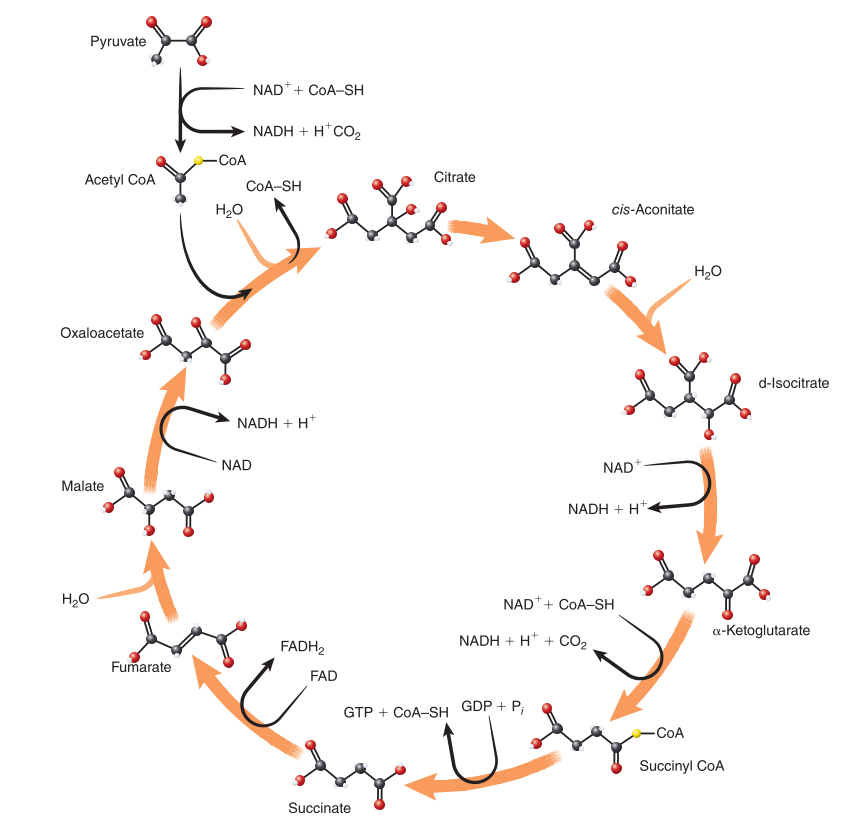
\includegraphics[width=0.6\linewidth]{figures/krebs.png}
    \end{center}
    \item These molecular alterations have the following important consequences:
    \begin{itemize}
        \item Two carbons are sequentially removed from the six-carbon citric acid molecule, converting it back into the \emf{four-carbon oxaloacetic acid}, which is now available at the top of the cycle to pick up another acetyl CoA (ferris wheel analogy)
        \item The released carbon atoms, which were originally present in the acetyl CoA that entered the cycle, are converted into two molecules of $CO_2$, which is passed out of the cell, into blood, and out through respiratory system.
        \item Hydrogen atoms are removed during four of the steps. The key purpose of the citric acid cycle is to produce these hydrogens for entry into the \emf{electron transport chain}. They are caught by \emf{nicotinamide adenine dinucleotide} ($NAD^+$) and \emf{flavine adenine dinucleotide} ($FAD$), converting them to $NADH$ and $FADH_2$.
        \item One more molecule of ATP is produced for each molecule of acetyl CoA processed. To be more precise, the released energy in the cycle is able to transform \emf{guanosine diphosphate} (GDP) to \emf{guanosine triphosphate} (GTP). The released energy is then used to turn ADP into ATP.
    \end{itemize}
\end{itemize}
\subsubsection{Electron Transport Chain}
\begin{itemize}
    \item The ``big payoff'' comes when $NADH$ and $FADH_2$ enter the \emf{electron transport chain}, which consists of electron carrier molecules located in the inner mitochondrial membrane lining the cristae.
    \item The high-energy electrons are extracted from the hydrogens held in $NADH$ and $FADH_2$ and are transferred from one electron-carrier molecule to another, within the cristae membrane, in an assembly line.
    \item $NADH$ and $FADH_2$ are converted back to $NAD^+$ and $FAD$. These molecules are now free to pick up more hydrogen atoms.
    \item While high-energy electrons are moved down the ETC, some energy is used to pump hydrogen ions within the intermembrane space. It is this accumulation of hydrogen ions that leads to the generation of ATP through the \emf{chemiosmotic mechanism.}
    \item The enzyme \emf{ATP synthase} is located within inner mitochondrial membrane, and is activated by the flow of hydroge ions back into the matrix from the inner mitochondrial membrane. Once activated, ATP synthase creates ATP from ADP and inorganic phosphate through \emf{oxidative phosphorylation.}
    \item The amount of ATP that can be produced depends on where they enter the electron transport chain. NADH enters early and can produce 3 ATP, while $FADH_2$ enters later and only produces $2$ ATP.
    \begin{center}
        \includegraphics[width=0.6\linewidth]{figures/etc.png}
    \end{center}
    \item Overall process can produce 30-32 ATP.
\end{itemize}
\subsubsection{Anaerobic Conditions}
\begin{itemize}
    \item Above discussion focuses on \emf{aerobic} metabolism. If oxygen levels are insufficient, \emf{anerobic} metabolism becomes the predominant source of energy.
    \item While glycolysis doesn't need oxygen, pyruvate decarboxylation does. If oxygen is not present, 2 NADH is used to produce 2 lactic acid. A total of only 2 ATP is generated. 
\end{itemize}
\subsubsection{ATP for Synthesis, Transport, and Mechanical Work}
\begin{itemize}
    \item Cell activites that require energy fall into three categories:
    \begin{itemize}
        \item \textit{Synthesis of new chemical compounds}: such as protein synthesis by the ER. Some cells (especially those with high rate of secretion and cells in the growth phase) use up to $75\%$ of the ATP they generate just to synthesize new compounds.
        \item \textit{Membrane transport}: such as the selective transport of molecules across membranes through active transport.
        \item \textit{Mechanical Work:} such as contraction of heart muscle to pump blood or the contraction of skeletal muscles to lift an object. 
    \end{itemize}
\end{itemize}
\subsection{Plasma Membrane}
\begin{itemize}
    \item For every cell, the membrane serves three important purposes:
    \begin{itemize}
        \item The cell's survival
        \item Ability to maintain homeostasis
        \item Ability to function cooperatively and in coordination with surrounding cells.
    \end{itemize}
\end{itemize}
\subsubsection{Membrane Structure and Composition}
\begin{itemize}
    \item Plasma membrane has a \emf{trilaminar structure} (two dark layers separated by a light middle layer).
    \item Membrane consists of a phospholipid bilayer. \emf{Phospholipids} have a polar head containing a negatively charged phosphate group and two non-polar fatty acids. The head is \emf{hydrophilic} and the tail is \emf{hydrophobic}.
    \item The bilayer is fluid in nature. They are not held together by strong chemical bonds, so they can swirl around rapidly as well as move about within their own half of the layer. This accounts for a large part for membrane fluidity.
    \item \emf{Cholesterol} contributes to both the fluidity and the stability.  Cholesterol are tucked in between phospholipid molecules, where they prevent fatty acid chains from packing together and crystallizing. Their spatial relationship with phospholipid molecules helps stabilize their positions.
    \item \emf{Membrane proteins} are attached to or inserted within the lipid bilayer. Some extend through the entire thickness of the membrane, while others only stand on the outer or inner surface anchored by interactions with a protein that span the membrane or by attachment to the lipid bilayer.
    \item The view of membrane structure is known as the \emf{fluid mosaic model,} in reference to the membrane fluidity and the ever changing mosaic pattern of proteins embedded within the lipid bilayer.
    \item The plasma membrane is \emf{sugar coated} by small amounts of membrane carbohydrates on the outer surface. Short-chained carbohydratees (like tiny antennas) protrude from the outer surface, bound mainly to membrane proteins and some to lipids. These sugary combinations are known as \emf{glycoproteins} and \emf{glycolipids} respectively.
    \item Different components of the plasma membrane serve three purposes:
    \begin{itemize}
        \item Lipid bilayer acts as barrier to diffusion
        \item Proteins perform specialized functions
        \item Carbohydrates act as self-recognition molecules for cell-to-cell interaction.
    \end{itemize}
\end{itemize}
\subsubsection{Lipid Bilayer}
\begin{itemize}
    \item Lipid bilayer has three important functions:
    \begin{itemize}
        \item Forms basic structure of membrane
        \item Hydrophobic interior serves as barrier to passage of water-soluble substances since they cannot dissolve in and pass through the bilayer.
        \item It is responsible for the fluidity of the membrane.
    \end{itemize}
\end{itemize}
\subsubsection{Membrane Proteins}
\begin{itemize}
    \item Membrane proteins serve the following specialized functions:
    \item Some span the membrane to form water filled channels. Water-soluble substance small enough to enter a channel can pass through the membrane this way.
    \begin{itemize}
        \item Only small ions can fit as channel can be as small as $0.8\text{ nm}$ in diameter.
        \item A given channel can selectively attract or repel particular ions. For example, only sodium can pass through sodium channels, and only potassium and pass through potassium channels.
        \item Seductiveness is due to specific arrangements of chemical groups on the interior of these channel walls.
        \item A given channel may close or open as a result to some controlling mechanism.
    \end{itemize}
    \item Proteins can also serve as \emf{carrier molecules}, which transfer specific substances across the membrane. The process is described in a later section.
    \item Proteins can be \emf{docking-marker acceptors} that bind in a lock-and-key fashion with the docking markers of secretory vesicles.
    \begin{itemize}
        \item Secretion is initiated when stimulatory signals trigger the fusion of the plasma membrane through interactions between these matching labels.
        \item The secretory vesicle subsequently opens up and empties its contents to the outside by exocytosis.
    \end{itemize}
    \item Proteins can also serve as \emf{membrane-bound enzymes} that control specific chemical reactions at either the inner or outer cell surface.
    \item Many proteins on the outer surface serve as \emf{receptor sites} that recognize and bind with specific molecules in the cell's environment.
    \item Many proteins on the outer membrane, in conjunction with carbohydrates, are able to recognize ``self'' (i.e. cells of the same type) and participate in cell-to-cell interactions.
\end{itemize}
\subsubsection{Self Recognition}
\begin{itemize}
    \item Short sugar chains on the outer membrane surface serve as self-identity markers that allows cells to interaction with each other:
    \begin{itemize}
        \item Different cells have different marks.
        \item Carbohydrate-containing surface markers are also involved in tissue growth. Typically, cells do not trespass across the boundaries of neighboring cells (with the exception of cancer).
    \end{itemize}
\end{itemize}
\subsection{Cell-to-Cell Adhesion}
\begin{itemize}
    \item Cells are held together by three different means:
    \begin{enumerate}
        \item The extracellular matrix
        \item Cell adhesion molecules in the cell's plasma membranes
        \item Specialized cell junctions
    \end{enumerate}
\end{itemize}
\subsubsection{Biological Glue}
\begin{itemize}
    \item Cells are held together by the \emf{extracellular matrix (ECM),} a mesh of proteins embedded in a gel-like substance composed of complex carbohydrates.
    \item Within the \emf{interstitial fluid} are three types of protein fibres
    \begin{itemize}
        \item \emf{Collagen} forms cable-like fibres that provide tensile strength
        \item \emf{Elastin} is a rubber-like protein fibre most abundant in tissues that need to stretch and recoil (i.e. in lungs)
        \item \emf{Fibronectin} promotes cell adhesion and holds cells in position
    \end{itemize}
    \item The ECM is secreted by local cells present in the matrix. Most of this abundant matrix in connective tissue is secreted by \emf{fibroblasts}.
    \item Note the ECM is not just passive scaffolding: it helps regulate the behaviour and functions of the cells with which it interacts.
\end{itemize}
\subsubsection{Cell Junctions}
\begin{itemize}
    \item Cells within given types of tissues are linked by one of the tree types of specialized cell junctions
    \begin{itemize}
        \item Desmosomes (adhering junctions) 
        \item Tight junctions (impermeable junctions)
        \item Gap junctions (communicating junctions)
    \end{itemize}
\end{itemize}
\subsubsection{Desmosomes}
\begin{itemize}
    \item \emf{Desmosomes} anchor together two adjacent but nontouching cells. It consists of two components: 
    \begin{itemize}
        \item A pair of dense, button-like cytoplasmic thickenings known as \emf{plaque}, located on the inner surface of each of the two adjacent cells
        \item Strong glycoprotein filaments containing cadherins (a type of CAM) that extend across the space between the two cells and attach to the plaque on both sides.
        \begin{center}
            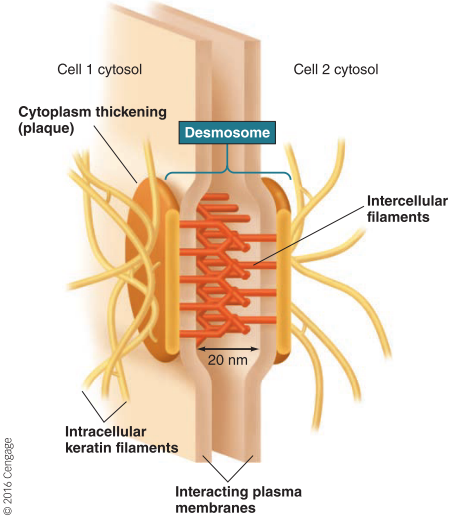
\includegraphics[width=0.5\linewidth]{figures/desmosome.png}
        \end{center}
        \item They are most abundant in tissues subject to considerable stretching, such as in skin, heart, and the uterus.
    \end{itemize}
\end{itemize}
\subsubsection{Tight Junctions}
\begin{itemize}
    \item At \emf{tight junctions,} adjacent cells firmly bind with each other at points of direct contact to seal off the passageway between two cells. They are found primarily in sheets of epithelial tissue.
    \begin{center}
        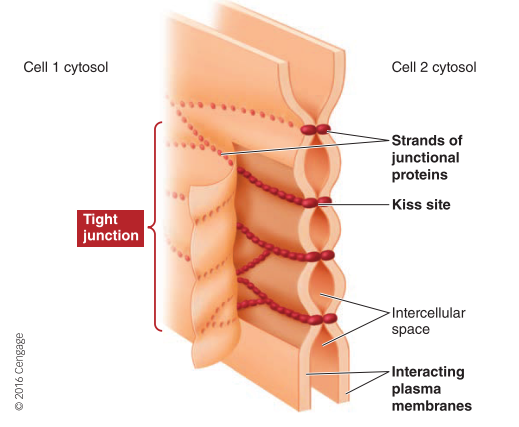
\includegraphics[width=0.5\linewidth]{figures/tight_junction.png}
    \end{center}
    \item All epithetlial sheets serve as highly selective barriers between two compartments that have considerably different chemical compositions.
    \item Lateral edges of adjacent cells are joined in a tight seal near their luminal border by \emf{kiss sites}, sites of direct fusion of \emf{junctional proteins} on the outer surfaces.
    \item Passage across the epithelial barrier must take place through the cells, not between them.
\end{itemize}
\subsubsection{Gap Junctions}
\begin{itemize}
    \item At a \emf{gap junction}, a gap exists between adjacent cells, which are linked by small, connecting tunnels formed by connexons.
    \item A \emf{connexon} is made up of six protein subunits arranged in a hollow tube-like structure.
    \item Two connexons extend outward, one from each of the plasma membranes of two adjacent cells, and join end to end to form the connecting tunnel between two cells.
    \item Gap junctions are communicating junctions. The small diameter allows small, water-soluble particles to pass between.
    \item They are abundant in cardiac muscle and smooth muscle
\end{itemize}
\subsection{Unassisted Membrane Transport}
\subsubsection{Passive Diffusion of Particles}
\begin{itemize}
    \item Understand how \emf{diffusion} works.
    \item Some examples:
    \begin{itemize}
        \item Oxygen is transferred across the lung membrane by diffusion. The blood carried to the lungs is low in oxygen, having given up oxygen to body tissues for metabolism. The air in the lungs are high in oxygen. Net diffusion of oxygen occurs into the blood as blood flows through the lungs.
    \end{itemize}
\end{itemize}
\subsubsection{Passive Diffusion of Ions}
\begin{itemize}
    \item An \emf{electrical gradient} occurs when there is a difference in charge between two adjacent areas.
    \item When both a chemical and electrical gradient is present, it is known as an \emf{electrochemical gradient}, and contributes to electrical properties of the plasma membrane.
\end{itemize}
\subsubsection{Osmosis}
\begin{itemize}
    \item Membrane protein forms \emf{aquaporins}, which are channels used for passage of water.
    \item \emf{Osmotic pressure} is a measure of the dendency for water to move into that solution because of its relative concentration of nonpenetrating solutes and water.
    \item At equilibrium, the net pressure (osmotic and hydrostatic) is zero.
\end{itemize}
\subsubsection{Tonicity}
\begin{itemize}
    \item When a solution surrounds the cell, the \emf{tonicity} of the solution is the effect the solution has on cell volume (i.e. does the cell swell or shrink?)
    \item An \emf{isotonic solution} has the same concentration of nonpenetrating solutes as normal body cells do.
    \item \emf{Hypotonic solutions} have a solution with below-normal concentration of nonpenetrating solutes.
    \item \emf{Hypertonic solutions} have a solution with above-normal concentration of nonpenetrating solutes.
\end{itemize}
\subsection{Assisted Membrane Transport}
\begin{itemize}
    \item Because large, poorly lipid-soluble molecules cannot cross plasma membrane on their own, the cell provide mechanisms for deliberately transporting these types of molecules. They use:
    \begin{itemize}
        \item Carrier-Mediated Transport: for small water-soluble substances
        \item Vesicular transport for movement of large molecules and multimolecular particles
    \end{itemize}
\end{itemize}
\subsubsection{Carrier-Mediated Transport}
\begin{itemize}
    \item Carrier proteins span the thickness of plasma membrane and can reverse shape so that specific binding sites can alternately be exposed at either side, known as \emf{flip-flops}
    \item During \emf{Carrier-mediated transport}, molecules attach to a binding cell within the interior of the carrier on one side of the membrane, causing the carrier to flip. After it moves away, the passenger detaches and the carrier reverts to original shape.
    \begin{center}
        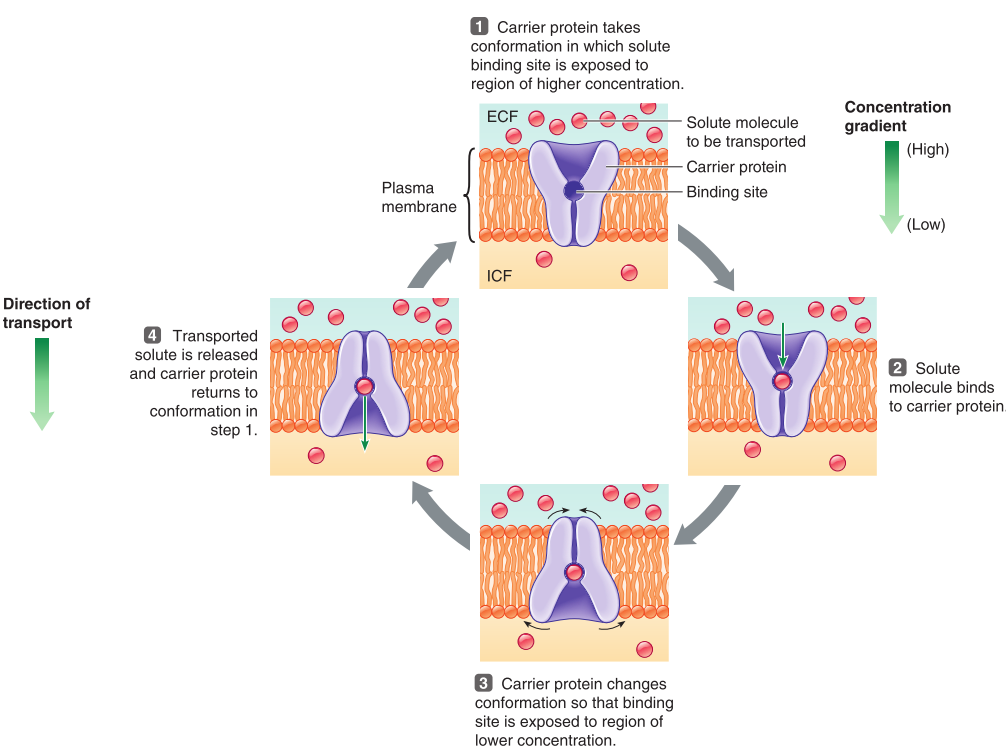
\includegraphics[width=0.8\linewidth]{figures/carrier_transport.png}
    \end{center}
    \item There are three important characteristics that determine the kind/amount of material that can be transferred: specificity, saturation, and competition
    \item For \emf{specificity}, each carrier protein is specialized to transport a specific substance or at most a few closely related chemical compounds.
    \item For \emf{saturation}, a limited number of carrier binding sites are available for a specific substance, creating a limit known as the \emf{transport maximum} ($T_m$). Before this is reached, the number of occupied binding sites is proportional to concentration.
    \item For \emf{competition}, several closely related compounds may compete for a ride across the membrane on the same carrier. If a given binding site can be occupied by more than one type of molecule, the rate of transport of each substance is less when both molecules are present than when either is present by itself.
\end{itemize}
\subsubsection{Active Transport}
\begin{itemize}
    \item \emf{Active transport} involves the use of a protein carrier to transfer a specific substance, but against the concentration gradient.
    \item Energy in the form of ATP is required to alter the relative affinity of the binding site when exposed one side of the plasma membrane or to the other.
    \item The binding site has a greater affinity for its passenger on the low-concentration side due to \textit{phosphorylation} of the carrier. The carrier splits the terminal phosphate from an ATP molecule. This reaction causes the carrier protein to flip. The change in shape is accompanied by \textit{dephosphorylation}, where the phosphate group is removed.
    \item Active transport mechanisms are often called \emf{pumps.}
    \item One important pump is the \emf{sodium-postassium pump}. This pump transports sodium ions out of the cell and picks up potassium from the outside. It moves three $Na^+$ out for every two $K^+$ it pumps in. This is important because:
    \begin{itemize}
        \item It establishes $Na^+$ and $K^+$ concentration gradients across the plasma membrane for all cells. These gradients are critically important in the ability of nerve and muscle cells to generate electrical signals.
        \item It helps regulate cell volume by controlling the concentrations of solutes inside the cell, minimizing osmotic effects.
        \item The energy used to run this pump also indirectly serves as the energy source for the cotransport of glucose and amino acids across intestinal and kidney cells. This process is known as \emf{secondary active transport}.
    \end{itemize}
    \begin{center}
        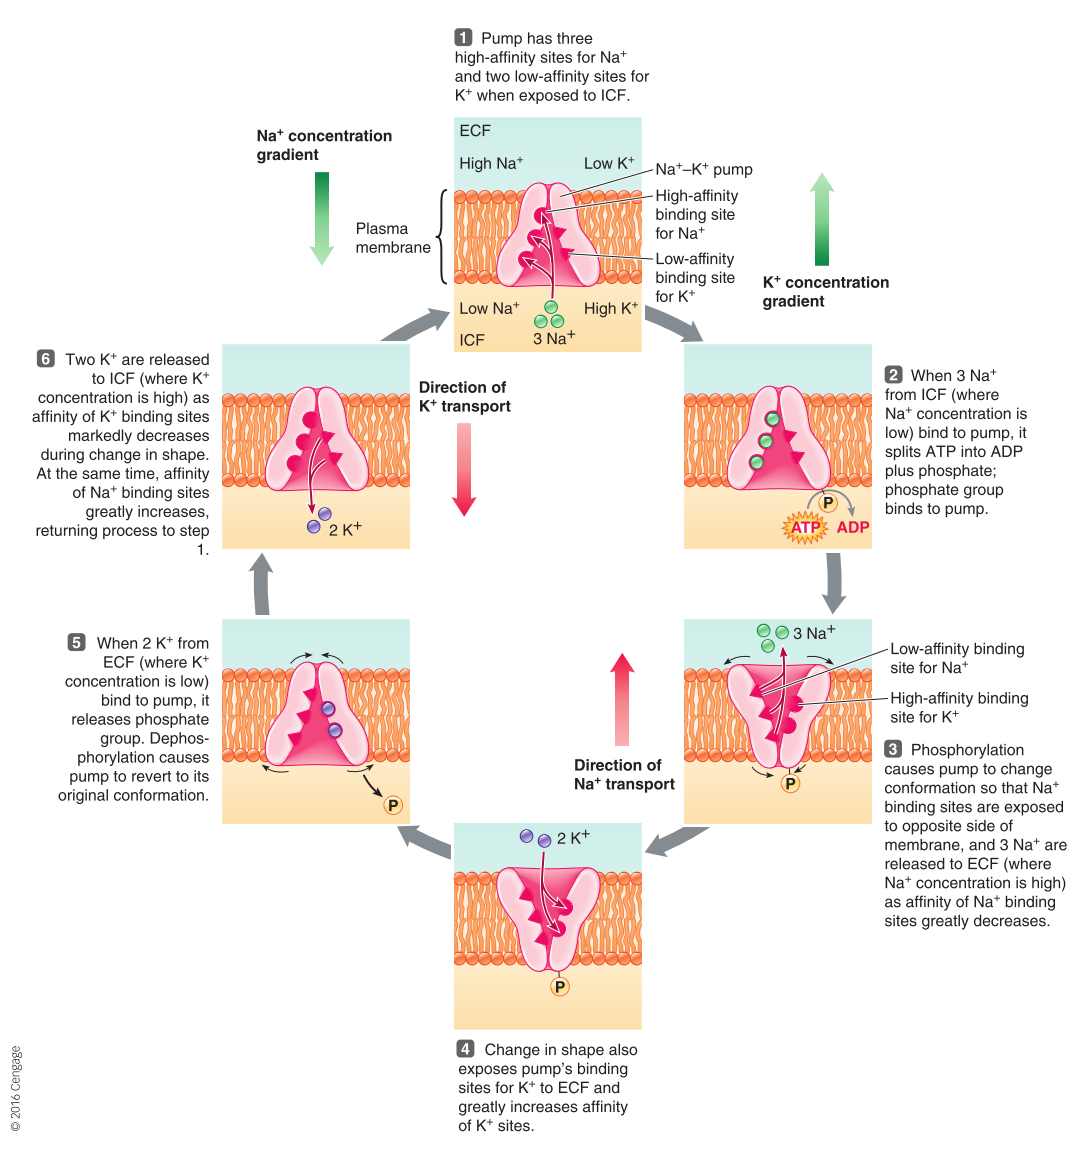
\includegraphics[width=0.7\linewidth]{figures/sodium_postassium_pump.png}
    \end{center}
\end{itemize}
\subsubsection{Secondary Active Transport}
\begin{itemize}
    \item Unlike most cells, intestinal and kideny cells actively transport glucose and amino acids from low to high from the intestinal lumen into the blood.
    \item Energy is not directly supplied to the carrier in \emf{secondary active transport}. Instead, the carriers are \emf{cotransport carriers} as they have two binding sites, one for $Na^+$ and one for the nunurient molecule.
    \item More $Na^+$ is in the lumen than inside the cells because the sodium-potassium pump transports sodium out of the cell, keeping the intracellular sodium concentration low.
    \begin{center}
        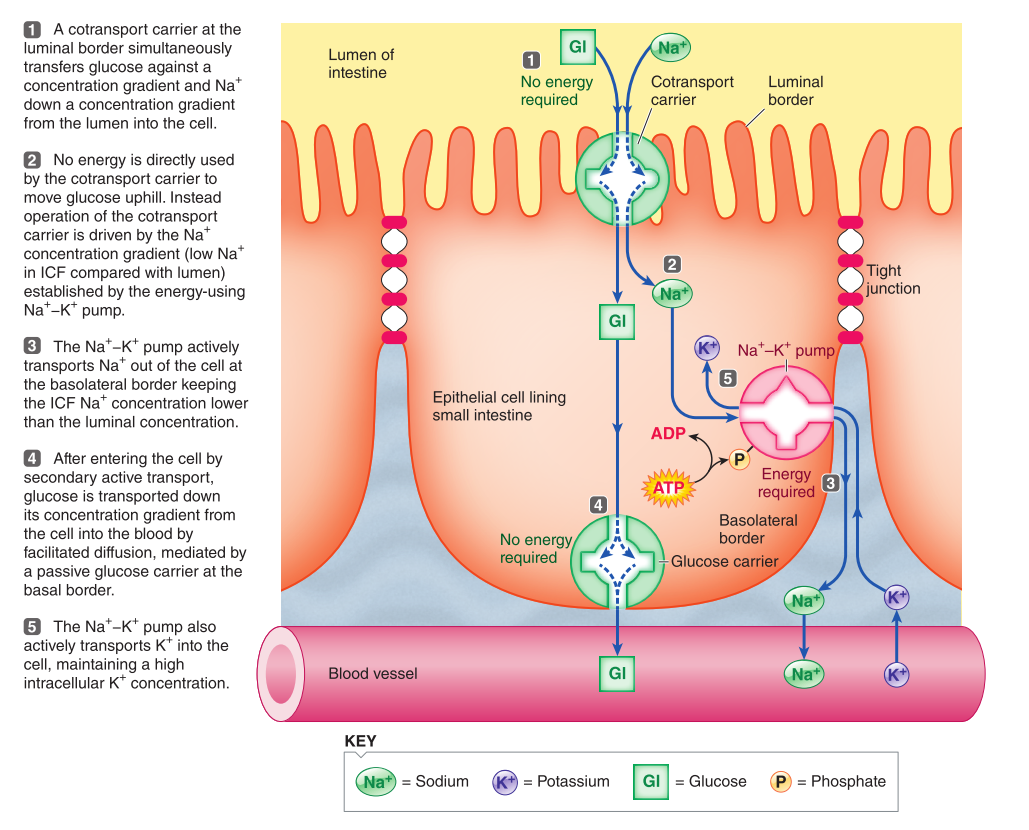
\includegraphics[width=0.8\linewidth]{figures/secondary_active_transport.png}
    \end{center}
\end{itemize}
\subsubsection{Vesicular Transport}
\begin{itemize}
    \item Large particles can be transferred between ICF and ECF not by crossing the membrane but by being wrapped in a membrane-enclosed vesicle, via \emf{vesicular transport.}
    \item Transport into the cell is \emf{endocytosis} while transport out of the cell is \emf{exocytosis}
\end{itemize}
\subsubsection{Endocytosis}
\begin{itemize}
    \item In \emf{endocytosis}, the membrane surrounds the substance, fuses over the surface, and pinching off a membrane enclosed vesicle so that the substance is trapped.
    \item Once inside the cell, the engulfed vesicle has two possible destinies:
    \begin{itemize}
        \item (Most common) Lysosomes fuse with vesicle to degrade and release contents into ICF
        \item (Sometimes) Bypass lysosomes and travel to opposite side, releasing its contents through exocytosis.
    \end{itemize}
    \item There are three different form of endocytosis
    \item With \emf{pinocytosis} (cell drinking), a small droplet of extracellular fluid is internalized. First, the membrane dips inwards.
    \item \emf{Receptor-mediated endocytosis} is a highly selective process that enables cells to import specific large molecules that it needs. This is triggered by a specific molecule binding to a surface membrane receptor site.
    \item During \emf{phagocytosis} (cell eating), large multimolecular particles are internalized. Only a few specialized cells are capable of this.
    \begin{center}
        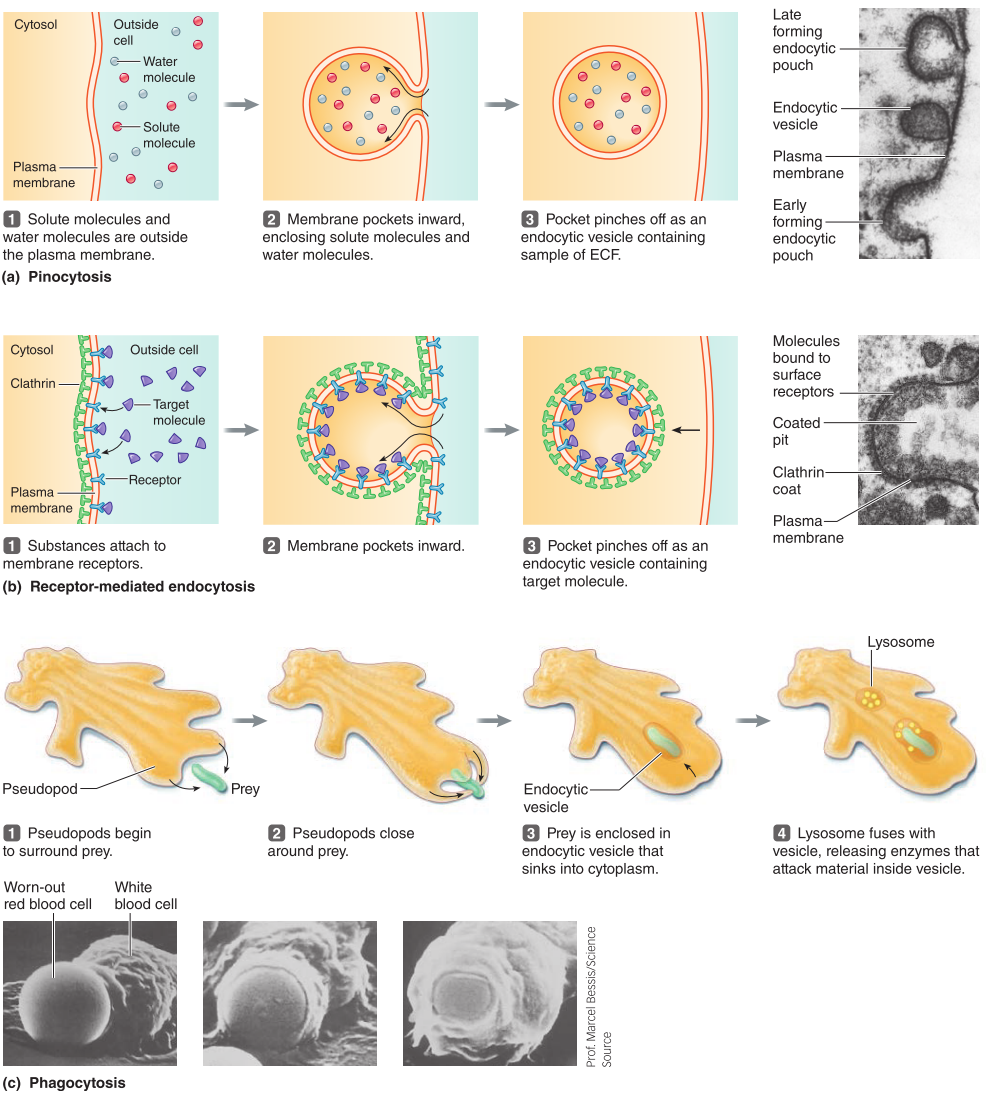
\includegraphics[width=0.8\linewidth]{figures/endocytosis.png}
    \end{center}
\end{itemize}
\subsubsection{Exocytosis}
\begin{itemize}
    \item \emf{Exocytosis} is almost the exact reverse of endocytosis. Materials packaged for export by the ER and Golgi complex are externalized by exocytosis, which serves two purposes:
    \begin{itemize}
        \item Provides a mechanism for secreting large polar molecules such as protein hormones and enzymes.
        \item Enables cell to add specific components to the membrane, such as selected carrier, channels, or receptors.
    \end{itemize}
\end{itemize}
\subsubsection{Secretory Vesicles}
\begin{itemize}
    \item In order for the Golgi complex to direct finished proteins to the proper destinations by wrapping them in membranes containing different surface protein molecules, which serves as a \emf{docking marker.}
    \item In secretory cells, numerous large \emf{secretory vesicles} (which contain the proteins to be secreted), bud off from the Golgi stacks. They remain stored until cell is stimulated by a signal that indicates a need for release of that particular secretory product.
    \item Secretory vesicles fuse only with the plasma membrane, preventing dangerous discharge into organelles.
    \item The membrane proteins serve three important functions:
    \begin{itemize}
        \item Specific proteins on the interior surface of the membrane act as \emf{recognition markers} for the recognition and attraction of specific molecules that have been processed in the golgi lumen. Newly finished proteins destined for secretion contain a sequence of amino acids called a \emf{sorting signal,} which ensures the proper cargo is captured and packaged within a secretory vesicle.
        \item \emf{Coat proteins} from the cytosol bind with another specific protein facing the outer surface of the membrane, which causes the surface membrane of the Golgi sac to curve and form a dome-shaped bud around the captured cargo. Eventually, the surface membrane closes and pinches off the vesicle.
        \item After budding off, the vesicle sheds its coat proteins. This uncoating exposes the docking markers known as \emf{v-SNARE}s, can link in a lock-and-key fashion with another protein marker, a \emf{t-SNARE,} found only on the targeted membrane.
    \end{itemize}
    \item Contents of secretory vesicles never come into contact with cytosol.
    \begin{center}
        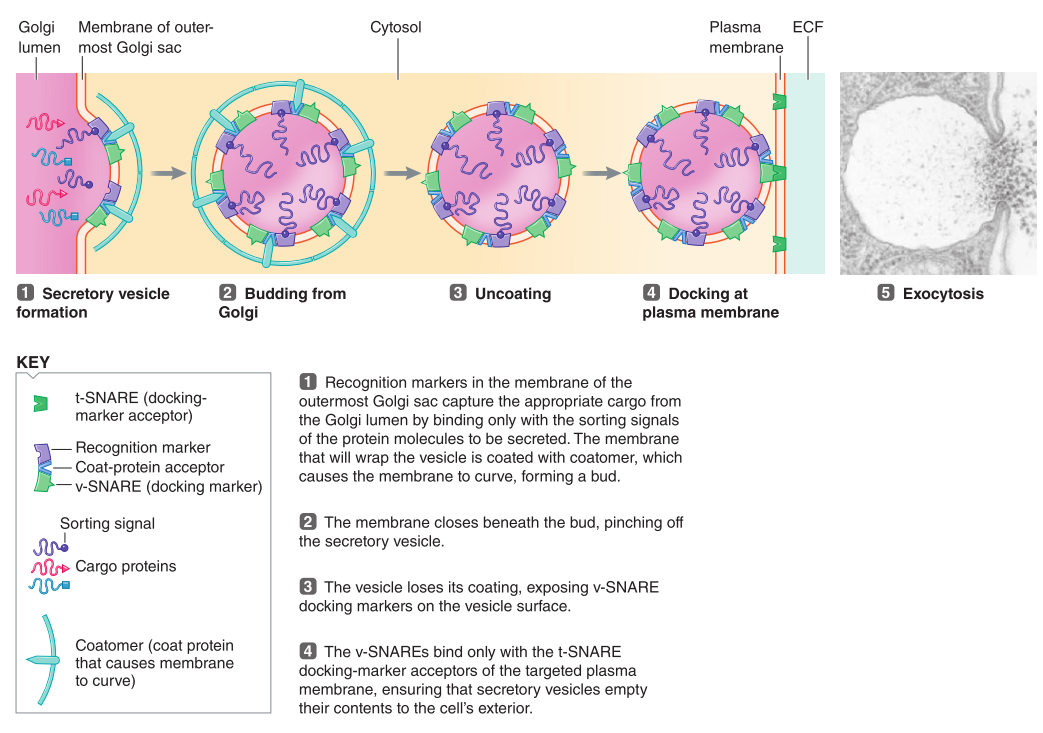
\includegraphics[width=0.9\linewidth]{figures/secretory_vesicles.png}
    \end{center}
\end{itemize}
\subsection{Intercellular Communication}
\subsubsection{Communication Between Cells}
\begin{itemize}
    \item Intracellular communication can take place in the following ways:
    \begin{itemize}
        \item Gap junctions allow exchanging of small ions and molecules.
        \item Identifying markers on surface membranes permits cells to directly link up
        \item The most common way is indirectly through extracellular chemical messengers. A specific chemical messenger is synthesized by specialized cells. On being released into the ECF by appropriate stimulation, they act on the messenger's \emf{target cells}.
    \end{itemize}
    \item There are four types of chemical messengers:
    \begin{itemize}
        \item \emf{Paracrines} are local chemical messengers whose effect is exerted only on neighboring cells in the immediate environment of their site of secretion.
        \item Neurons communicate directly with the cells they innervate by releasing \emf{neurotransmitters}, which are very short-ranged chemical messengers, in response to electrical signals.
        \item \emf{Hormones} are long-range chemical messengers that are specifically secreted into the blood by endocrine glands in response to an appropriate signal. The blood carries the messengers to other sites in the body, where they exert their effects on their target cells some distance away from their site of release.
        \item \emf{Neurohormones} are hormones released into the blood by \emf{neurosecretory neurons.} Instead of directly innervating target cells. Similar to endocrine cells, neurosecretory neurons release blood-borne chemical messengers, whereas ordinary neurons secret short-range neurotransmitters into a confined space. 
    \end{itemize}
    \begin{center}
        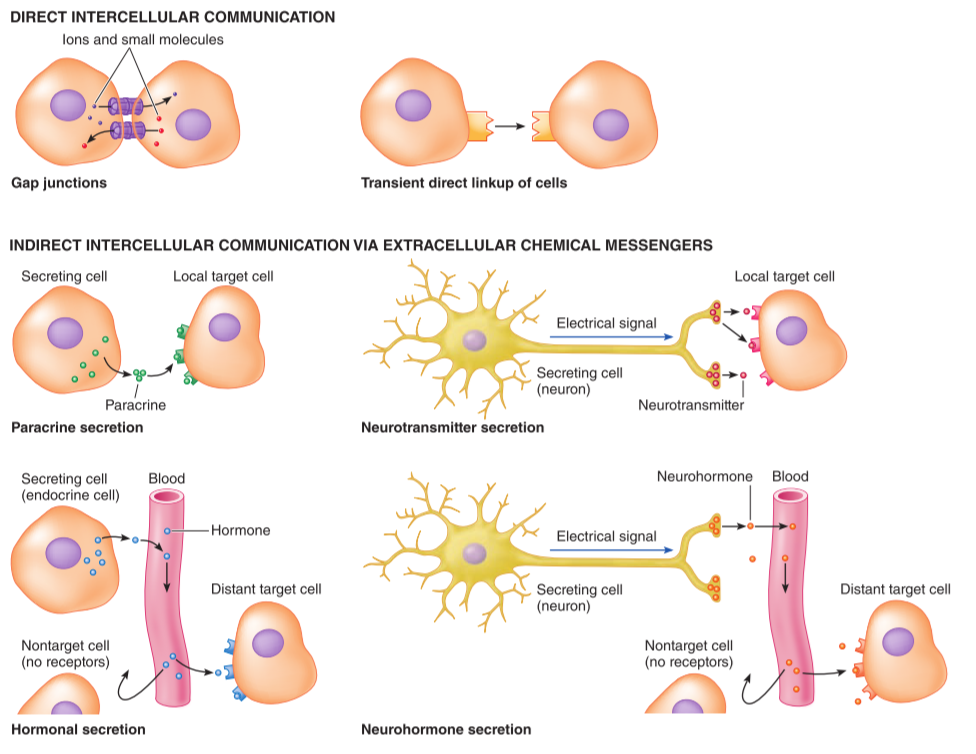
\includegraphics[width=0.8\linewidth]{figures/communication.png}
    \end{center}
\end{itemize}
\subsubsection{Signal Transduction}
\begin{itemize}
    \item \emf{Signal transduction} refers to the process by which incoming signals are conveyed to the target cell's interior for execution.
    \item Lipid-soluble extracellular chemical messengers gain entry into the cell by dissolving in and passing through the lipi bilayer. They then bind to receptors inside the target cell and initiate the desired response themselves.
    \item Extracellular chemical messengers that are water-soluble cannot gain entry to the target cell through the lipid bilayer. They signal the cell by first binding with surface membrane receptors specific for that given messenger, triggering a sequence of events that controls a particular cellular activity.
    \item There are two ways in which the extracellular messenger, known as the \emf{first messenger} when bound to its matching receptor can produce the desired response:
    \begin{itemize}
        \item By opening or closing channels
        \item By activating second-messenger systems
    \end{itemize}
\end{itemize}
\subsubsection{Chemically Gated Channels}
\begin{itemize}
    \item Some examples of chemically gated channels:
    \begin{itemize}
        \item Opening of chemically gated channels in the subsynaptic membrane of neuron in response to binding of neurotransmitters: The resultant small, short-lived movement of charge-carrying ions across the membrane through these open channels generates electrical signals.
        \item Stimulation of muscle cells: Chemically gated channels open in response to the binding of neurotransmitters released from neurons.
    \end{itemize}
    \item On completion, the messenger is removed from the receptor site and the chemically gated channel close. The ions that moved across the membrane through opened channels to trigger the response are returned to their original location by special membrane carriers.
\end{itemize}
\subsubsection{Second-Messenger Pathways}
\begin{itemize}
    \item The binding of the first messenger to a receptor can serve as a signal for activating an intracellular \emf{Second messenger,} which relays orders through a series of biochemical intermediaries to particular intracellular proteins that carry out the dictated response, such as changes in cellular metabolism or secretory activity.
    \item Second-messenger systems are widely used throughout the body, including being one of the key means by which most water-soluble hormones ultimately bring about their effects.
\end{itemize}
\subsection{Membrane Potential}
\subsubsection{Concentration and Permeability of Ions}
\begin{itemize}
    \item \emf{Membrane potential} refers to the difference in electrical potential between inside and outside a cell, typically measured in millivots.
    \item Cells of excitable tissues have the ability to produce rapid, transient changes in their membrane potential when excited, producing electrical signals.
    \item When electrical signals are not produced, the membrane potential is known as the \emf{resting membrane potential}
    \item Knowledge of the relative concentrations and permeability of ions allow us to analyze the forces across the plasma membrane, which includes the following few sections.
\end{itemize}
\subsubsection{Effects of \texorpdfstring{$K^+$}{K+} Movement on \texorpdfstring{$K^+$}{K+} Membrane Equilibrium Potential}
\begin{itemize}
    \item There are two opposing forces acting on $K^+$: the concentration gradient tending to move $K^+$ out of the cell, and the electrical gradient tending to move these ions into the cell.
    \item Eventually, the equilibrium potential of $K^+$ will be reached and the potential at this point is known as the \emf{$K^+$ equilibrium potential} ($E_{K^+}$)), which is equal to $-90\text{ mV}.$
    \item By convention, the sign always designates the polarity of the excess charge on the inside of the membrane. So a negative potential means that the inside of the cell is more negatively charged.
    \item The equilibrium potential for a given ion of differing concentrations across a membrane can be calculated using the \emf{Nernst equation},
    \begin{equation}
        E = \frac{RT}{zF}\ln\frac{C_0}{C_1} = (61\text{ mV})\log\frac{C_o}{C_i},
    \end{equation}
    where $z$ is the ion's valence ($+1$ for $K^+$ and $Na^{+}$). $C_o$ is the concentration outside and $C_i$ is the concentration inside.
    \begin{center}
        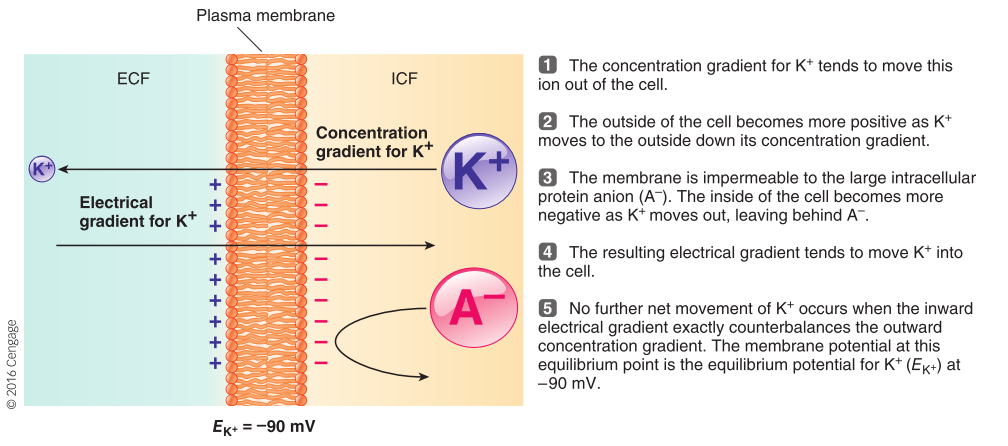
\includegraphics[width=0.8\linewidth]{figures/potassium_equilibrium.png}
    \end{center}
\end{itemize}
\subsubsection{Effects of \texorpdfstring{$Na^+$}{Na+} Movement on \texorpdfstring{$Na^+$}{Na+} Membrane Equilibrium Potential}
\begin{itemize}
    \item A similar effect happens for the movement of $Na^+$ alone, which creates a build up of negative charges outside, primarily in the form of chloride.
    \item Because the concentration gradient of $Na^+$ is not as large as that for potassium, the equilibrium membrane potential for sodium is $E_{Na^+}$ is $60\text{ mV}$, which is not as great as potassium.
\end{itemize}
\subsubsection{Concurrent \texorpdfstring{$K^+$}{K+} and \texorpdfstring{$Na^+$}{Na+} Effects on Membrane Potential}
\begin{itemize}
    \item However, neither potassium nor sodium exists alone, so the previous two examples were purely hypothetical. 
    \item The greater the permeability of the plasma membrane ofr a given ion, the greater is the tendency for that ion to drive the membrane potential toward the ion's own equilibrium potential. Because rest membrane is 50-75 times as permeable to $K^+$ as to $Na^+$, potassium influences the resting membrane potential to a greater extent.
    \begin{center}
        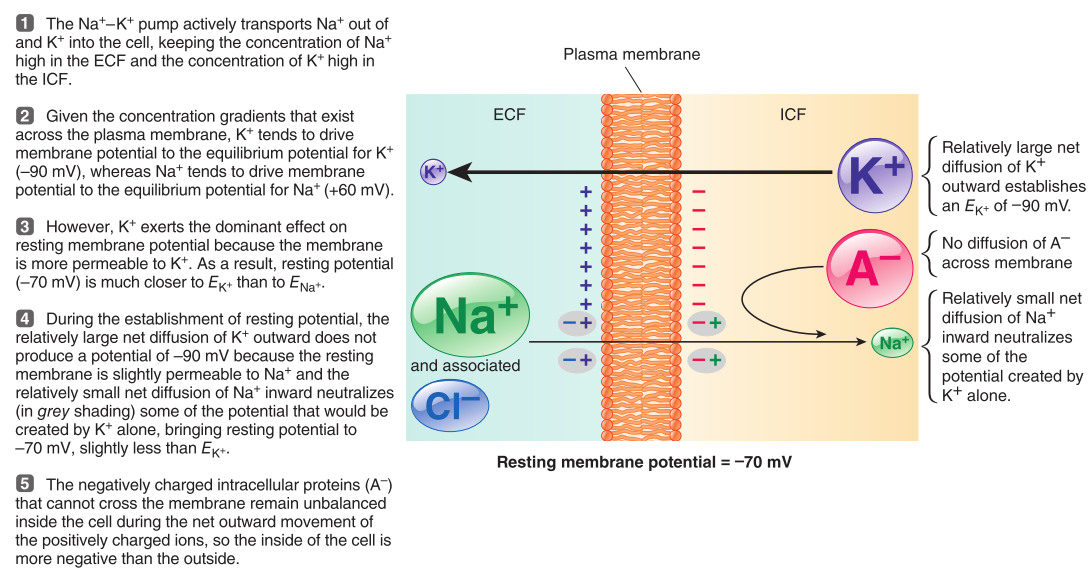
\includegraphics[width=0.8\linewidth]{figures/potassium_sodium_equilibrium.png}
    \end{center}
    \item To account for all effects, we use the \emf{Goldman-Hodgkin-Katz Equation}, which says the membrane potential is
    \begin{equation}
        V_m = \frac{RT}{zF}\ln\left(\frac{P_{Na}[Na^+]_o+P_K[K^+]_o+P_{Cl}[Cl^-]_i}{P_{Na}[Na^+]_i+P_K[K^+]_i+P_{Cl}[Cl^-]_o}\right)
    \end{equation}
    where $P_i$ is the selectivity for ion $i$.
    \item The resting membrane potential is actually $E=-70\text{ mV}.$
\end{itemize}
\subsubsection{Chloride Movement at Resting Membrane Potential}
\begin{itemize}
    \item The chloride ion, is the principal ECF anion with an equilibrium potential of $-70\text{ mV}$, exactly the same as the resting membrane potential. The membrane potential is responsible for driving the distribution of chloride across the membrane.
    \item Most cells are highly permeable to chloride but have no pumps for this ion, so the distribution is mainly passive. In this case, chloride is driven out of the cell, establishing an inward concentration gradient that exactly counterbalances the outward electrical gradient.
\end{itemize}
\subsubsection{Specialized Use of Membrane Potential in Nerve and Muscle Cells}
\begin{itemize}
    \item Nerve and muscle cells have developed a specialized use for membrane potential. These cells can rapidly and transiently alter their membrane permeabilities to specific ions in response to appropriate simulation, bringing about fluctuation.
    \item Because of this, they are considered \emf{excitable tissues} because, when excited, they change their resting potential to produce electrical signals.
\end{itemize}
\subsubsection{Depolarization and Hyperpolarization}
\begin{itemize}
    \item We introduce some vocabulary related to describing changes in potential:
    \item \emf{Polarization:} Charges are separated across the membrane, so the membrane has potential. Any time the value of the membrane potential is nonzero, the membrane is in a state of polarization.
    \item \emf{Depolarization:} The resting potential becomes less negative.
    \item \emf{Repolarization:} The membrane returns to resting potential after having being depolarized.
    \item \emf{Hyperpolarization:} The membrane becomes more polarized than at resting potential.
\end{itemize}
\subsubsection{Electrical Signals and Ion Movement}
\begin{itemize}
    \item Changes in membrane potential are brought about by changes in ion movement across the membrane. Changes in ion movement, in turn, are brought about by changes in membrane permeability in response to \emf{triggering events}. Depending on the type of electrical signal, a triggering event might be:
    \begin{itemize}
        \item A change in electrical field in the vicinity
        \item An interaction of a chemical messenger with a surface receptor
        \item A stimulus, such as sound waves stimulating specialized nerve cells
        \item Spontaneous change of potential caused by inherent imbalances in the leak-pump cycle.
    \end{itemize}
    \item Because water-soluble ions cannot penetrate the lipid bilayer, these charge can cross only through membrane channels which can either be \emf{leak channels} or \emf{gated channels.}
    \item \emf{Leak channels} are open all the time.
    \item \emf{Gated channels} have gates that can alternately be open or close. This opening/closing results from a change in the shape of the protein that forms the gated channel. There are four types of gated channels, depending on what factor induces that change in shape:
    \begin{itemize}
        \item \emf{Voltage-gated channels:} open or close in response to changes in membrane potential
        \item \emf{Chemically-gated channels:} change conformation in response to the binding of a specific chemical messenger to a membrane receptor in close association with the channel.
        \item \emf{Mechanically-gated channels:} respond to stretching or other mechanical deformation
        \item \emf{Thermally-gated channels:} which responds to local changes in temperature
    \end{itemize}
\end{itemize}
\subsection{Graded Potential}
\subsection{Action Potential}
\subsection{Regeneration of Nerve Fibers}
\subsection{Synapses}
\end{document}